\documentclass[UTF8]{ctexart}
%\setmainfont{Noto Sans CJK SC}
\usepackage{xeCJK}
\setCJKmainfont[BoldFont=Noto Sans S Chinese Bold Bold]{Noto Sans S Chinese Regular}
\usepackage{amsmath}
\usepackage{geometry}
\geometry{a4paper, left=2cm, right=2cm,top=2cm,bottom=2cm}
\usepackage{pifont}
%\ding{172}=\textcircled{1}
\usepackage{booktabs}
\usepackage{hyperref}
\usepackage{esint}
\usepackage{mathrsfs}
\usepackage{graphicx}
\usepackage{wrapfig}
\usepackage{float}
\usepackage[perpage]{footmisc}
\newcommand*{\dif}{\mathop{}\!\mathrm{d}}
\renewcommand{\thefootnote}{\ding{\numexpr171+\value{footnote}}}

\title{Part1 Fundermental}
\author{Xiao Liang}
\date{\today}


\begin{document}
	\maketitle
	\numberwithin{equation}{section}
	\tableofcontents
	\newpage
	%\CJKfontspec{Noto Sans Mono CJK SC}
	\CJKfontspec[BoldFont=Noto Sans S Chinese Bold Bold]{Noto Sans S Chinese Regular}
	
	\section{第一原理}
	(波动)光学的第一原理便是麦克斯韦方程组,结合物质方程可以得到所有的波动光学结论。
	
	\subsection{麦克斯韦方程组}
	
\noindent 积分表达式

	\begin{equation}
	\begin{aligned}
	\oiint \boldsymbol{D} \cdot \dif \boldsymbol{\sigma}&=Q
	\\
	\oiint \boldsymbol{B} \cdot \dif \boldsymbol{\sigma}&=0
	\\
	\oint \boldsymbol{E} \cdot \dif \boldsymbol{l}&=-\iint \frac{\partial \boldsymbol{B}}{\partial t} \dif \sigma
	\\
	\oint \boldsymbol{H} \cdot \dif \boldsymbol{l}&=\boldsymbol{I}+\iint \frac{\partial D}{\partial t} \dif \boldsymbol{\sigma}
	\\
	\end{aligned}
	\end{equation}
	
\noindent 微分表达式

\begin{equation}
	\begin{aligned}
	\nabla \cdot \boldsymbol{D}&=\rho
	\\
	\nabla \cdot \boldsymbol{B}&=0
	\\
	\nabla \times \boldsymbol{E}&=-\frac{\partial \boldsymbol{B}}{\partial t}
	\\
	\nabla \times \boldsymbol{H}&=\boldsymbol{j}+\frac{\partial \boldsymbol{D}}{\partial t}
	\\
	\end{aligned}\label{equ_Maxwell}
\end{equation}

	\subsection{物质方程}
	物质方程是没法从第一原理导出而需要通过实验方可确定的具有物质特异性(特异性通常体现在某些系数上)的方程。波动光学理论中的物质方程如下:
	
	\begin{equation}
		\boldsymbol{D}=\varepsilon \boldsymbol{E}, \quad \boldsymbol{B}=\mu \boldsymbol{H}, \quad \boldsymbol{j}=\sigma \boldsymbol{E}
	\end{equation}
	
	结合麦克斯韦方程组便可以推导出波动光学所有的结论。
	
	\section{光的波动性}
	光本质就是电磁场,可视为束缚在原子中的电子类似电偶极子进行振荡发出的变化的电磁场,该电磁场具备波动性。可以通过麦克斯韦方程组证明。
	
	利用麦克斯韦方程组\ref{equ_Maxwell}的第三、第四式,考虑没有自由电荷和自由电流的情形,并结合场论公式
	\begin{equation}
		\nabla \times(\nabla \times \boldsymbol{E})=\nabla(\nabla \cdot \boldsymbol{E})-\nabla^{2} \boldsymbol{E}
	\end{equation}
	
\noindent 可以得到:
\begin{equation}
	\begin{aligned}
	\nabla^{2} \boldsymbol{E}-\frac{1}{v^{2}}\frac{\partial^{2} \boldsymbol{E}}{\partial t^{2}}&=0
	\\
	\nabla^{2} \boldsymbol{H}-\frac{1}{v^{2}}\frac{\partial^{2} \boldsymbol{H}}{\partial t^{2}}&=0
	\end{aligned}\label{equ_wave}
\end{equation}
	这表明电场和磁场以波动的形式传播,速度为$ v=\frac{1}{\sqrt{\varepsilon \mu}} $
	
	定义电磁波在传播介质中的绝对折射率
	\begin{equation}
		n=\frac{c}{v}=\sqrt{\frac{\varepsilon \mu}{\varepsilon_{0} \mu_{0}}}=\sqrt{\varepsilon^{\prime} \mu^{\prime}}
	\end{equation}
	
\noindent 其中$ \varepsilon^{\prime} $和$ \mu^{\prime} $分别称为相对介电常数和相对磁导率。

	\section{电磁波的简单解}
	方程组\ref{equ_wave}有几个简单解,也是波动光学使用最多的几个情况。
	
	\subsection{平面波}
	平面波是波阵面为平面的波,该平面与传播方向垂直。波阵面是波在介质中传播时,经相同时间所到达的各点所连成的直线、曲线(二维内)或面(三维内),是相位相同点的集合。最前方的曲面称为\textbf{波前}。
	
	平面波的数学表达形式为:
	\begin{equation}
		\tilde{\psi}(\boldsymbol{x}, t)=\tilde{A} e^{i(\boldsymbol{k} \cdot \boldsymbol{x}-\omega t)}
	\end{equation}
	
\noindent 平面波是从遥远的地方发出的光波,是一种近似处理。

	\subsubsection{平面电磁波的性质}
	1、电磁波是横波
	
	考虑$ \nabla \cdot \boldsymbol{E} = i \boldsymbol{k} \cdot \boldsymbol{E} $和$ \nabla \cdot \boldsymbol{E} = 0 $可以得到
	\begin{equation}
		\boldsymbol{k} \cdot \boldsymbol{E} = 0
	\end{equation}
	
\noindent 这表明,电场波动是横波,电矢量的振动方向恒垂直于波的传播方向。同理可以得到磁场的类似结论。

	2、$ \boldsymbol{E} $和$ \boldsymbol{B} $互相垂直
	
	考虑$ \nabla \times \boldsymbol{E} = - \frac{\partial \boldsymbol{B}}{\partial t} $和电场与磁场的平面波表达式可以得到
	\begin{equation}
		\boldsymbol{B} = \sqrt{\varepsilon \mu} \boldsymbol{k}_{0} \times \boldsymbol{E}\label{equ_E_B}
	\end{equation}
	
	3、$ \boldsymbol{E} $和$ \boldsymbol{B} $同向
	
	由式子\ref{equ_E_B}可得到
	\begin{equation}
		\frac{|\boldsymbol{E}|}{|\boldsymbol{B}|}=\frac{1}{\sqrt{\varepsilon \mu}}=v
	\end{equation}
	
\noindent 由于$ \boldsymbol{E} $和$ \boldsymbol{B} $的振幅之比为一正实数,所以两矢量振动始终同位相,电磁波传播时它们同步变化。

	\subsection{球面波和柱面波}
	球面波是波阵面为球面的波。球面的法向方向即为波的传播方向。
	
	球面波的数学表达形式为
	\begin{equation}
		E=\frac{A_{1}}{r} e^{-i(\omega t-k \boldsymbol{r})}
	\end{equation}
	
\noindent 球面波是一个点光源所发出的光波。

	柱面波则是波阵面为柱面的波,是线光源发出的光波,数学表达形式为
	\begin{equation}
		E=\frac{A_{1}}{\sqrt{r}} e^{-i(\omega t-k \boldsymbol{r})}
	\end{equation}
	
	\section{光的产生和传播}
	
	\subsection{光辐射的经典模型}
	光的产生可以理解为物体辐射电磁波的过程。暂且只考虑原子发光的情况,经典电磁场理论把原子发光看做是原子内部形成的电偶极子的辐射。在外界能量的激发下,由于原子核和电子的剧烈运动和相互作用,原子的正负电中心常不重合,从而形成了一个振荡电偶极子,于是在周围空间产生交变的电磁场,即辐射出光波。
	
	\subsection{辐射能}
	电磁场的能量密度为
	\begin{equation}
	W=\frac{1}{2} \varepsilon E^{2}+\frac{1}{2} \mu H^{2}
	\end{equation}
	
	为了描述电子能量的传播,因此\textbf{辐射矢量},又称\textbf{坡印廷矢量S},该矢量大小等于单位时间内通过垂直于传播方向的单位面积的电磁能量,矢量的方向取能量的流动方向。可以得到
	\begin{equation}
	S=w v=\frac{v}{2}\left(\varepsilon E^{2}+\mu H^{2}\right)
	\end{equation}
	
\noindent 即
\begin{equation}
\boldsymbol{S}=v \varepsilon E^{2}=v \mu H^{2}=\boldsymbol{E} \cdot \boldsymbol{H}
\end{equation}

	对坡印廷矢量在一段时间内求平均可知:\textbf{电偶极子辐射强度的平均值与电偶极子振荡的振幅平方成正比,与辐射的电磁波的频率的四次方成正比(与波长的四次方成反比)}。
	
	考虑平面波可以得到简单的形式
	\begin{equation}
		\overline{S}=\frac{1}{2} v \varepsilon A^{2} = \frac{1}{2} \sqrt{\frac{\varepsilon}{\mu}} A^{2}
	\end{equation}
	
	通常将辐射强度的平均值称为光强度,在只需要求相对强度的情况下,可以忽略比例系数,得到
	\begin{equation}
		I=A^{2}
	\end{equation}
	
	\subsection{电磁场的边值关系}
	运用麦克斯韦方程组\ref{equ_Maxwell}和在分界面上做小圆柱、长方形的方法可以得到以下的边值关系
	\begin{equation}
	\begin{aligned}
	\boldsymbol{n} \cdot \left(\boldsymbol{B}_{1} - \boldsymbol{B}_{2}\right) &= 0
	\\
	\boldsymbol{n} \cdot \left(\boldsymbol{D}_{1} - \boldsymbol{D}_{2}\right) &= 0
	\\
	\boldsymbol{n} \times \left(\boldsymbol{E}_{1} - \boldsymbol{E}_{2}\right) &= 0
	\\
	\boldsymbol{n} \times \left(\boldsymbol{H}_{1} - \boldsymbol{H}_{2}\right) &= 0
	\end{aligned}
	\end{equation}
	
	\subsection{反射定律和折射定律}
	只考虑电场,因为磁场情况与之几乎一模一样。考虑入射场、反射场和折射场$ \boldsymbol{E_{1}}, \boldsymbol{E_{1}^{\prime}}, \boldsymbol{E_{2}} $以及边值条件$ \boldsymbol{n} \times \left(\boldsymbol{E}_{1}+\boldsymbol{E}_{1}^{\prime}\right) = \boldsymbol{n} \times \boldsymbol{E} _{2}$可以得到
	\begin{equation}
		\omega_{1} = \omega_{1}^{\prime} = \omega_{2}
	\end{equation}
	
\noindent 这表明入射波、反射波和折射波的频率相同。又由于边值条件对整个分界面上的位置矢量都成立,所以在整个界面有
\begin{equation}
	\boldsymbol{k}_{1} \cdot \boldsymbol{r} = \boldsymbol{k}_{1}^{\prime} \cdot \boldsymbol{r} = \boldsymbol{k}_{2} \cdot \boldsymbol{r}
\end{equation}

\noindent 由此可知$ \boldsymbol{k}_{1}, \boldsymbol{k}_{1}^{\prime}, \boldsymbol{k}_{2} $三者共面,同在入射面内。

	根据上述结论很容易推知$ \theta_{1} = \theta_{1}^{\prime} $,即\textbf{反射角等于入射角}以及$ n_{1} \sin \theta_{1} = n_{2} \sin \theta_{2} $,即\textbf{折射定律}。
	
	\subsection{菲涅耳公式}
	菲涅耳公式指出了反射光、折射光和入射光的振幅和位相关系。
	
	考虑将入射光分解为电矢量(磁矢量的处理与之类似)垂直于入射面和平行于入射面的s波和p波。
	
	\subsubsection{s波的反射系数和透射系数}
	根据边值关系可以得到:
	\begin{equation}
	\begin{aligned}
	E_{1s}+E_{1s}^{\prime} &= E_{2s}
	\\
	H_{1p}\cos \theta_{1} - H_{1p}^{\prime} \cos \theta_{1} &= H_{2p} \cos \theta_{2}
	\end{aligned}
	\end{equation}
	
\noindent 考虑到$ \mu \approx \mu_{0} $和$ H_{p} = n \sqrt{\frac{\varepsilon_{0}}{\mu_{0}}} E_{s} $并代入电场的平面波方程,并利用折射定律得到:
\begin{equation}
	\begin{aligned}
	r_{s} = \frac{A_{1s}^{\prime}}{A_{1s}} &= - \frac{\sin \left(\theta_{1}-\theta_{2}\right)}{\sin \left(\theta_{1}+\theta_{2}\right)}
	\\
	t_{s} = \frac{A_{2s}}{A_{1s}} &= \frac{2 \sin \theta_{2} \cos \theta_{1}}{\sin \left(\theta_{1} + \theta_{2}\right)}
	\end{aligned}
\end{equation}

\noindent $ r_{s} $和$ r_{p} $称为s波的反射系数和透射系数。

	\subsubsection{p波的反射系数和透射系数}
	同理由边值关系可得
	\begin{equation}
	\begin{aligned}
	E_{1p} \cos \theta_{1} - E_{1p}^{\prime} \cos \theta_{1} &= E_{2p} \cos \theta_{2}
	\\
	H_{1s} + H_{1s}^{\prime} &= H_{2s}
	\end{aligned}
	\end{equation}
	
\noindent 利用$ H_{1s} = n_{1} E_{1p} $和折射定律并代入平面波的表达式可得
\begin{equation}
	\begin{aligned}
	r_{p} &= \frac{A_{1p}^{\prime}}{A_{1p}} = \frac{\tan \left(\theta_{1} - \theta_{2}\right)}{\tan \left(\theta_{1} + \theta_{2}\right)}
	\\
	t_{p} &= \frac{A_{2p}}{A_{1p}} = \frac{2 \sin \theta_{2} \cos \theta_{1}}{\sin \left(\theta_{1} + \theta_{2}\right) \cos \left(\theta_{1} - \theta_{2}\right)}
	\end{aligned}
\end{equation}

\noindent $ r_{p} $和$ t_{p} $分别称为p波的反射系数和透射系数。

	\subsubsection{两种情况的菲涅耳公式讨论}
	分$ n_{1}<n_{2} $(光从光疏介质到光密介质)和$ n_{1}>n_{2} $(光从光密介质到光疏介质)两种情况进行讨论。
	
	\newpage
	对于第一种情况,如下图所示
	\begin{figure}[ht]
		\centering
		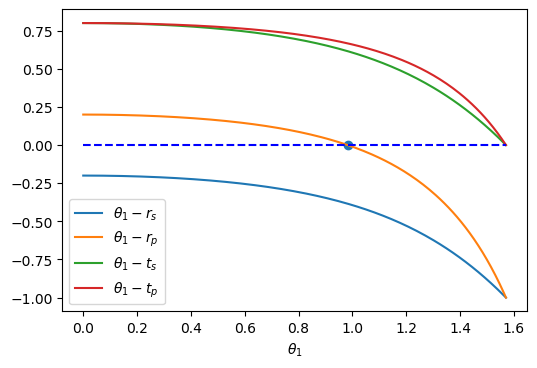
\includegraphics[width=12cm]{Fenier_equ1.png}
		\caption{光从光疏介质到光密介质的反射系数和透射系数随入射角的变化曲线}
		\label{figure_Fenier_equ1}
	\end{figure}

	由图\ref{figure_Fenier_equ1}可知,不管入射角$ \theta_{1} $为何值,$ r_{s} $总是负的,这说明对于s波,在界面上反射光总有$ \pi $的相位跃变。对于$ r_{p} $,则在$ \theta_{1}>\theta_{B} $时方存在$ \pi $的相位跃变。
	
	当平面波在接近正入射或掠入射下从光疏介质与光密介质的分界面反射时,反射光振动相对于入射光振动发生了$ \pi $的位相跃变。通常把反射时发生的$ \pi $相位跃变称为“半波损失”。
	
	对于第二种情况,如下图所示
		\begin{figure}[ht]
		\centering
		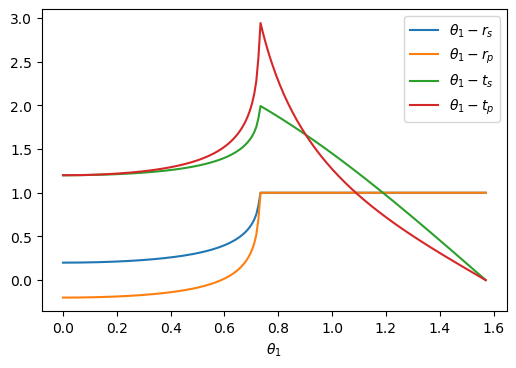
\includegraphics[width=12cm]{Fenier_equ2.png}
		\caption{光从光密介质到光疏介质的反射系数和透射系数随入射角的变化曲线}
		\label{figure_Fenier_equ2}
	\end{figure}

	可以有两点发现:
	
	(1) 入射角$ \theta_{1} \leq \theta_{C} $时,$ r_{s}, r_{p} $变为负数,但模值为1,这表示发生了全反射现象;
	
	(2) 在$ \theta_{1} < \theta_{C} $时,关于$ r_{s} $和$ r_{p} $的正负号的结论将与$ n_{1} < n_{2} $得到的结论相反,在$ n_{1} > n_{2} $的情况下反射光在界面上不会发生相位变化。
	
	\subsection{反射率和透射率}
	将入射波的强度记为$ I_{1} $,它表示单位时间内通过垂直传播方向的单位面积的能量。每秒入射到分界面单位面积上能量为:
	\begin{equation}
	W_{1}=I_{1} \cos \theta_{1}=\frac{1}{2} \sqrt{\frac{\varepsilon_{1}}{\mu_{1}}} A_{1}^{2} \cos \theta_{1}
	\end{equation}
	
	同理可得反射波和折射波每秒从单位面积带走的能量$ W_{1}^{\prime} $和$ W_{2} $因此,在分界面上反射波、折射波的能量流与入射波的能量流之比为:
	\begin{equation}
	\begin{aligned}
	R&=\frac{W_{i}^{\prime}}{W_{1}}=\frac{I_{1}^{\prime}}{I_{1}}=\frac{A_{1}^{\prime 2}}{A_{i}^{2}}
	\\
	T&= \frac{W_{2}}{W_{1}}=\frac{\sqrt{\frac{\varepsilon_{2}}{\mu_{2}} \cos \theta_{2} A_{2}^{2}}}{\sqrt{\frac{\varepsilon_{1}}{\mu_{1}} \cos \theta_{1} A_{1}^{2}}} = \frac{n_{2} \cos \theta_{2} A_{2}^{2}}{n_{1} \cos \theta_{1} A_{1}^{2}}
	\end{aligned}
	\end{equation}
	
\noindent 上式有用到对于非磁性介质的近似$ \mu_{1} \approx \mu_{2} $。$ R, T $分别称为反射率和折射率。利用菲涅耳公式可得光矢量垂直于入射面的偏振光的反射率和折射率:
\begin{equation}
	\begin{aligned}
	R_{s}&=\frac{\sin ^{2}\left(\theta_{1}-\theta_{2}^{\prime}\right)}{\sin ^{2}\left(\theta_{1}+\theta_{2}\right)}
	\\
	T_{s}&=\frac{n_{2} \cos \theta_{2}}{n_{1} \cos \theta_{1}} \cdot \frac{4 \sin ^{2} \theta_{2} \cos ^{2} \theta_{1}}{\sin ^{2}\left(\theta_{1}+\theta_{2}\right)}
	\end{aligned}
\end{equation}

\noindent 光矢量平行于入射面的偏振光的反射率和透射率为:
\begin{equation}
	\begin{aligned}
	R_{p}&=\frac{\tan ^{2}\left(\theta_{1}-\theta_{2}\right)}{\tan ^{2}\left(\theta_{1}+\theta_{2}\right)}
	\\
	T_{p}&=\frac{n_{2} \cos \theta_{2}}{n_{1} \cos \theta_{1}} \cdot \frac{4 \sin ^{2} \theta_{2} \cos ^{2} \theta_{1}}{\sin ^{2}\left(\theta_{1}+\theta_{2}\right) \cos ^{2}\left(\theta_{1}-\theta_{2}\right)}
	\end{aligned}
\end{equation}

	可以看出无论是哪个方向的分量,都有$ R+T=1 $,这说明在反射和折射时能量是守恒的。对于入射光是自然光的情况,每个分量的能量都等于入射光能量的一半。
	
	\subsection{反射和折射产生的偏振}
	当入射角满足$ \theta_{1} + \theta_{2}=\frac{\pi}{2} $,则有$ R_{p}=0 $,因而反射光是完全偏振的,其电矢量的振动垂直于入射面。这个结果通常称为\textbf{布儒斯特定律},而此时的入射角称为\textbf{起偏振角}或\textbf{布儒斯特角},记为$ \theta_{B} $.将$ \theta_{B}+\theta_{2}=\frac{\pi}{2} $,即可得到
	\begin{equation}
		\tan \theta_{B} = n \enspace (n=\frac{n_{2}}{n_{1}})
	\end{equation}
	
	当光波从光密介质射向光疏介质($ n_{2}<n_{1} $)时,会存在没有折射光的情况,这个时候入射光全部反射回介质1,这个现象称为\textbf{全反射}。满足
	\begin{equation}
		\sin \theta_{c} = \frac{n_{2}}{n_{1}}
	\end{equation}
	
\noindent 的入射角称为\textbf{临界角},对应的折射角为$ \frac{\pi}{2} $.

	在全反射情况下,反射光的光强始终等于入射光,但随着入射角的变化,存在相位的变化。
	
	\subsection{光的吸收、色散和散射}
	在金属中光的吸收主要来源于自由电子因为入射光波的作用形成电流,而电流在金属内将产生焦耳热,从而导致了光能的流失。在其他物质中光的吸收可以视作在入射光波作用下,介质中的束缚电子做受迫运动,而电子进行受迫振动会发射出次级波,次级波和入射波叠加成投射光波而射出介质。
	
	\subsubsection{吸收定律}
	介质的吸收形式上可以引入一个复折射率来描述(复数可以带来幅值变化效果)
	\begin{equation}
		\tilde{n} = n(1+i\kappa)
	\end{equation}
	
\noindent 则在介质内沿$ z $轴传播的平面波的电场可以写做
\begin{equation}
	\boldsymbol{E} = \boldsymbol{A} \exp \left[i \left(\frac{\omega \cdot \tilde{n}}{c} z - \omega t\right)\right]
\end{equation}

\noindent 由此得到平面波的强度
\begin{equation}
	I = I_{0} \exp (- \overline{\alpha} z)
\end{equation}

\noindent 该式通常称为\textbf{布朗尔定律}或\textbf{朗伯定律},其中$ \overline{\alpha} = 2 n \kappa \omega / c $称为物质的\textbf{吸收系数}。

	\subsubsection{吸收的波长选择性}
大多数物质的吸收具有波长选择性,对可见光进行选择吸收,会使白光变成彩色光。绝大部分物体呈现颜色,都是其表面或体内对可见光进行选择吸收的结果。

物质吸收的选择性可用它们的吸收系数和波长的关系曲线表示。在一定的波长范围内物质的吸收很强,而且有一个极大值,这个吸收范围称为\textbf{吸收带}。在带外的波长区域,物质的吸收很小,是透明区。一种物质往往有许多吸收带,并且彼此的形态可能相差很大。

固体和液体的吸收带比较宽,而稀薄气体的则很窄,变成了\textbf{吸收线}。这是因为在稀薄气体中,原子间的距离很大,它们之间的相互影响很小,原子内电子的振动可以认为不受周围原子的影响。每一种物质的原子系统的振动都有一些固有的振动频率,当入射光波的频率和这些固有振动频率一致时,就会引起共振,这时入射波的能量被强烈地吸收。

\subsubsection{光的色散}
光的色散是一种光在介质中传播时其折射率(或速度)随频率(或波长)而变的现象。存在正常色散和反常色散两种情况,两种情况的区分是相对的。

正常色散发生在物质透明区(在此区域内物质对光的吸收很小),其特点是,随着光的波长的增大,折射率减小,因而色散曲线是单调下降的,可以用经验公式,柯西色散公式来描述
\begin{equation}
n= a +\frac{b}{\lambda^{2}}+\frac{c}{\lambda^{4}}
\end{equation}

\noindent 反常色散发生在物质吸收区域,在该区域内,物质的折射率随波长的增大而增大。整个色散曲线一般是正常色散和反常色散分段组成的。

	\subsubsection{色散的经典理论}
	色散的经典理论把不同频率的光波在介质中以不同的速度传播理解为介电常数的不同,对于介电常数如何同频率产生联系,洛伦兹用经典电子论找到了它们之间的关系。
	
	先考虑稀薄气体介质的情况,设频率为$ \omega $的光波$ \boldsymbol{E} = \boldsymbol{A} \exp (- i \omega t) $入射到气体介质内,使介质内的束缚电子引起受迫振动。由于原子中电子速度相比光子很低,而光波磁场作用力比电场作用力低得多,因此可以忽略入射光波的磁场对电子的作用力。这样,电子受迫振动方程为
	\begin{equation}
	\frac{\dif^{2} \boldsymbol{l}}{\dif t} + \gamma \frac{\dif \boldsymbol{l}}{\dif t} + \omega_{0}^{2} \boldsymbol{l} = \frac{q}{m} \boldsymbol{A} \exp (-i \omega t) \label{equ_force}
	\end{equation}
	
	可设其解为
	\begin{equation}
	\boldsymbol{l}= \boldsymbol{l}_{0} \exp (-i \omega t)
	\end{equation}
	
	\noindent 代入\ref{equ_force}可得
	\begin{equation}
	\boldsymbol{l}_{0} = \frac{q \boldsymbol{A}}{m \sqrt{\left(\omega_{0}^{2}-\omega^{2}\right)}+\omega^{2} \gamma^{2}} \exp(i \delta)
\end{equation}

\noindent 其中,$ \tan \delta = \frac{\gamma \omega}{\omega_{0}^{2} - \omega^{2}} $.

	当外力频率与内在频率一致$ \omega = \omega_{0} $时,振动最大,即为\textbf{共振现象},这时简谐振子吸收光波能量最大。

	电子的振动将使原子成为一个振荡电偶极子,其电偶极矩为$ q \boldsymbol{l} $。设介质单位体积内有$ N $个原子,这样介质的极化强度为
	\begin{equation}
		\boldsymbol{P} = N q \boldsymbol{l} = \frac{N q^{2}}{m} \cdot \frac{\boldsymbol{E}}{\omega_{0}^{2} - \omega^{2} - i \gamma \omega}
	\end{equation}

\noindent 考虑到
\begin{equation}
	\boldsymbol{D} = \varepsilon \boldsymbol{E} = \varepsilon_{0} \boldsymbol{E} + \boldsymbol{P}
\end{equation}

\noindent 以及折射率定义
\begin{equation}
	\tilde{n}^{2} = \frac{\varepsilon}{\varepsilon_{0}}
\end{equation}

\noindent 得到色散公式
\begin{equation}
	\tilde{n}^{2} = 1 + \frac{N q^{2}}{\varepsilon_{0} m \left(\omega_{0}^{2} - \omega^{2} - i \gamma \omega\right)}
\end{equation}

	以上讨论假定电子的振动只有一个固有频率$ \omega_{0} $。实际上电子可以有若干个不同的固有频率,假设这些固有频率振动的概率分别为$ f_{1}, f_{2}, \cdots $,得到一般的色散公式
	\begin{equation}
		\tilde{n}^{2} = 1+ \frac{N q^{2}}{\varepsilon_{0} m} \sum_{j} \frac{f_{i}}{\left(\omega_{j}^{2} - \omega^{2} - i \gamma_{j} \omega\right)}
	\end{equation}
	
	这使得在每一个$ \omega = \omega_{j} $附近,对应有一个吸收带和反常色散区。在这些区域之外,是正常色散区。
	
	下面来看固体、液体和压缩气体中的情况。在这些情况下,由于原子和分子之间的距离很近,周围分子在光场作用下极化所产生的影响不可以再忽略,此时可以得到作用在电子上的电场为:
	\begin{equation}
		\boldsymbol{E}^{\prime} = \boldsymbol{E} + \frac{\boldsymbol{P}}{3 \varepsilon_{0}}
	\end{equation}
	
\noindent 做类似的推导可以得到在这种情况下的色散公式
\begin{equation}
	\frac{n^{2}-1}{n^{2}+2} = \frac{N q^{2}}{3 \varepsilon_{0} m \left(\omega_{j}^{2} - \omega^{2} - i \gamma_{j} \omega\right)}
\end{equation}

	\subsection{光的散射}
	\subsubsection{散射类型和来源}
	由于介质内存在折射率不同的悬浮微粒存在,使得即使不正对着入射光的方向,也能够清楚地看到光,这种现象称为光的散射。
	
	悬浮微粒的散射也称为\textbf{瑞利散射}。这种散射通常很强,散射光的强度与溶液的浓度和浑浊度有关。在非常纯净的气体和液体中,也可以观察到散射现象,这种散射现象被称为\textbf{分子散射},是由于分子的热运动导致介质的密度对一定的平均值的偏差。这种偏差造成折射率的变化,使介质的光学均匀性遭到破坏。
	
	散射现象的来源是介质的非均匀性导致入射光激发的次波的振幅不完全相同,彼此的相位也有差别,这样一来次波相干叠加的结果,除了一部分光波仍沿着反射和折射定律规定的方向传播外,在其他方向上不能完全抵消,造成散射光。
	
	\subsubsection{散射规律}
	散射光的强度与入射光波长的四次方成反比,即
	\begin{equation}
		I \propto \lambda^{-4}
	\end{equation}
	
\noindent 这一规律称为\textbf{瑞利散射定律},只适用于散射体比光波波长小的情形。对于大块物质的散射,瑞利定律不适用,这时散射光强度与波长的关系不大。当入射光是自然光时,散射光强度与观察方向有关,关系为
\begin{equation}
	I_{\theta} = I_{\frac{\pi}{2}} \left( 1 + \cos^{2} \theta\right)
\end{equation}
\end{document}
